\section{Solution}
In this section we will describe the solutions to the problems. This are the problems we will have to deal with: The physics of the bridge builder, the collapsing of the bridge and  the interface of the bridge builder.
\subsection{Physics}
We will use the physics engine in JMonkeyengine to keep track of the weight, gravity, location and maybe tractive force of each building blocks. This will make it easier to write an algorithm that decides when the bridge will break that also depends on the connections between the building blocks. We will try for each building blocks what mass and tractive force is most realistic and we will have to find a realistic weight for the train. 
\subsection{Collapsing of the Bridge}
JMonkeyEnginge handles collisions between building blocks by looking at the weight and gravity on each building block and this will result in a realistic collapsing bridge. However we still have to compute whether a building block breaks and we still have to visualize some special effects like smoke or fire.
\subsection{Interface}
We decided to keep the interface very simple. The current interface looks like \ref{fig:gui}. In this interface only 2 building blocks are available, but we hope to get some more. There are some simple buttons. The two building blocks, the undo button and the play button for letting the train ride over the bridge. By pressing the letter matched to the button, will result in that action too.
\begin{figure}[H]
    \centering
    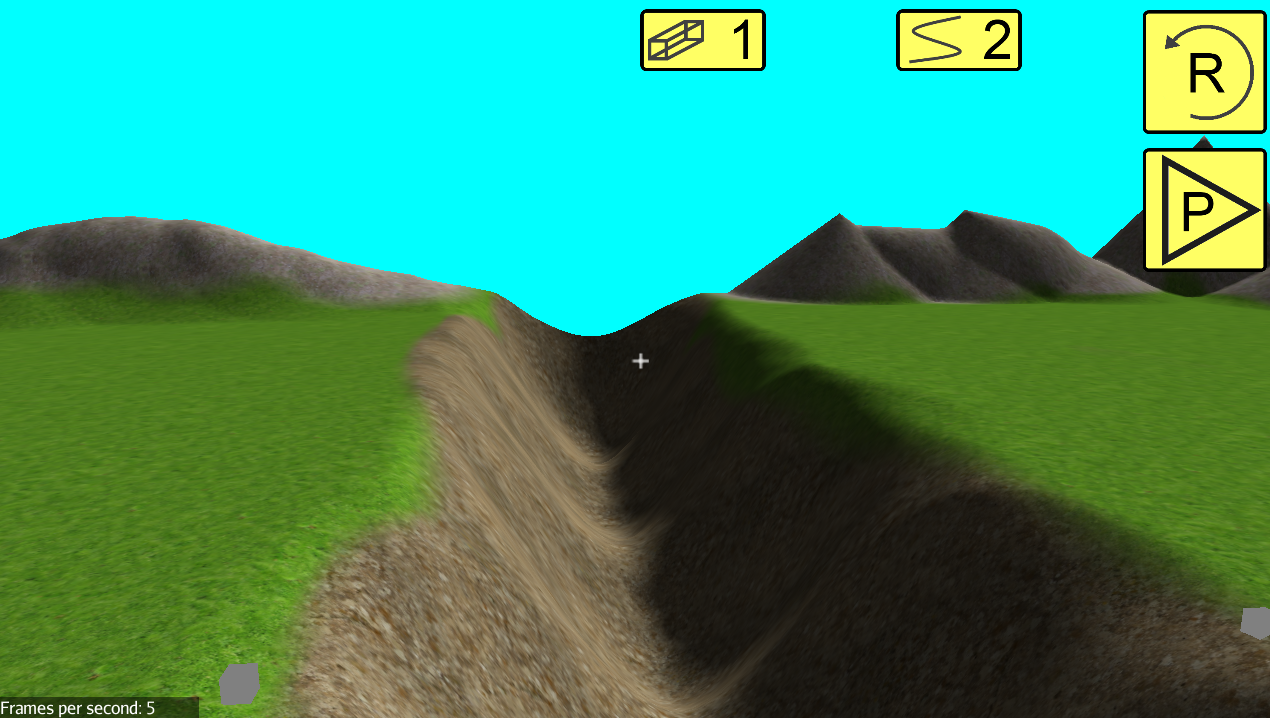
\includegraphics[width=0.8\textwidth]{screenshots/GUI.png}
    \caption{Current interface}
    \label{fig:gui}
\end{figure}
The user can click on a building block to select this building block. The selected building block will get another color as you can see in figure \ref{fig:bbs}. After that the user can select a point where he wants to connect the building block. This is shown in figure \ref{fig:scp}. When there is a connection point the user can select in which way the building block should be build. This is shown in figure \ref{fig:builded}.
\begin{figure}[H]
    \centering
    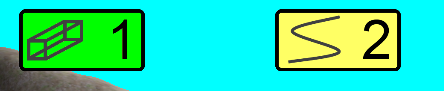
\includegraphics[width=0.4\textwidth]{screenshots/BuildingBlockSelected.png}
    \caption{Building block 1 is selected}
    \label{fig:bbs}
\end{figure}
\begin{figure}[H]
    \centering
    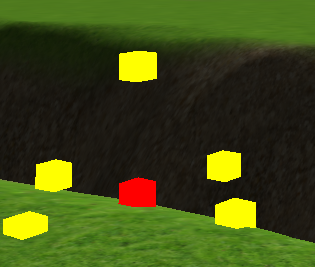
\includegraphics[width=0.4\textwidth]{screenshots/select.png}
    \caption{Selected connection point}
    \label{fig:scp}
\end{figure}
\begin{figure}[H]
    \centering
    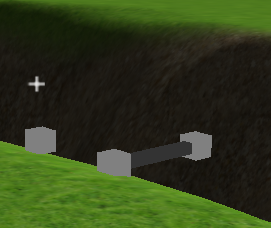
\includegraphics[width=0.4\textwidth]{screenshots/Builded.png}
    \caption{Building block is build}
    \label{fig:builded}
\end{figure}